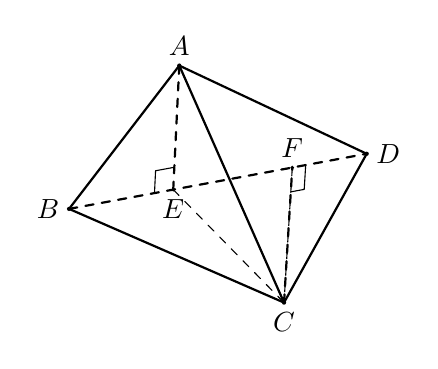
\begin{tikzpicture}[line cap=round,line join=round,scale=0.7]
\usetikzlibrary{calc}

% place points in a 2D perspective-like layout
\coordinate (B) at (0,0);
\coordinate (D) at (5.4,1.0);
\coordinate (C) at (3.9,-1.7);
\coordinate (A) at (2.0,2.6);

% E,F on BD (feet, schematic)
\coordinate (E) at ($(B)!0.35!(D)$);
\coordinate (F) at ($(B)!0.75!(D)$);

% faces edges (schematic)
\draw[thick] (B)--(A)--(D);
\draw[thick] (B)--(C)--(D);
\draw[thick] (A)--(C);

% fold line BD
\draw[dashed,thick] (B)--(D);

% perpendicular-ish segments (as in solution)
\draw[dashed,thick] (A)--(E);
\draw[dashed,thick] (C)--(F);

% auxiliary dashed inside
\draw[dashed] (E)--(C);
\draw[dashed] (F)--(C);

% right-angle marks at E,F (schematic)
\begin{scope}
  \coordinate (e1) at ($(E)!0.18!(B)$);
  \coordinate (e2) at ($(E)!0.18!(A)$);
  \coordinate (e3) at ($(e2)+(e1)-(E)$);
  \draw (e1) -- (e3) -- (e2);
\end{scope}
\begin{scope}
  \coordinate (f1) at ($(F)!0.18!(D)$);
  \coordinate (f2) at ($(F)!0.18!(C)$);
  \coordinate (f3) at ($(f2)+(f1)-(F)$);
  \draw (f1) -- (f3) -- (f2);
\end{scope}

% point marks + labels
\fill (A) circle (1.1pt) node[above] {$A$};
\fill (B) circle (1.1pt) node[left] {$B$};
\fill (C) circle (1.1pt) node[below] {$C$};
\fill (D) circle (1.1pt) node[right] {$D$};
\fill (E) circle (1.0pt) node[below] {$E$};
\fill (F) circle (1.0pt) node[above] {$F$};

\end{tikzpicture}